\textbf{COLUNI 2024 -- Questão 25}\par\medskip Leia o texto a seguir.

\begin{center}\textbf{Os riscos à saúde causados pelo uso de mercúrio no garimpo}\end{center}

\begin{center}
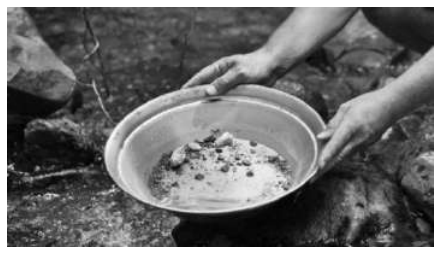
\includegraphics[width=0.32\linewidth]{static/simulados/coluni/figuras/2024/questao-25/figura-1.png}
\end{center}

\textbf{Bruna Alves}\\
\textbf{De São Paulo para BBC News Brasil}

Os garimpos ilegais, que usam mercúrio em excesso para viabilizar a separação do ouro dos demais sedimentos, causam a contaminação dos peixes, a morte dos rios, a remoção da cobertura vegetal e, consequentemente, a fuga dos animais. É o que tem ocorrido com os habitantes da Terra Indígena Yanomami, que fica entre os estados de Roraima e do Amazonas.

No caso da extração nos rios da Amazônia, por exemplo, o ouro está no ambiente em forma de partículas muito pequenas. O mercúrio metálico, nesse caso, é usado para uni-las, formando um amálgama (liga metálica) com o ouro, viabilizando a sua separação de outros componentes.

Disponível em: https://www.bbc.com/portuguese/articles/c7246ee619qo. Acesso em: 29 ago. 2023. (Adaptado)

Com base nas informações fornecidas e nos conhecimentos sobre ciências, analise as seguintes afirmativas:

I. O mercúrio apresenta ponto de fusão mais baixo que o do ouro.

II. O mercúrio e o ouro estão localizados na mesma coluna da Tabela Periódica.

III. O amálgama é classificado como uma substância pura.

IV. O processo de separação do ouro dos demais sedimentos, nos garimpos, utilizando-se o mercúrio, é chamado de centrifugação.

Está CORRETO o que se afirma em:
\begin{enumerate}
\item I, apenas.
\item I, II e III, apenas.
\item II e IV, apenas.
\item III e IV, apenas.
\end{enumerate}
